\renewcommand{\familydefault}{\sfdefault}

\title{AMVARA DASHBOARD}
\author{
        Amvara Consulting S.L.\\
}
\date{\today} %% Adds today date

\documentclass[12pt]{article}
\usepackage[legalpaper, margin=3cm]{geometry}
\usepackage{hyperref}
\usepackage{graphicx}
\usepackage{fancyhdr}
\graphicspath{ {.images/} }


\begin{document} %% Starts Document
\maketitle %% Prints title and author 
\begin{centering} %% Displays an image and webpage url centered
	
\includegraphics{amvara} \par
	\url{https://www.amvara.de} \par
\end{centering}
\newpage %% Page break

\section{Data Formats} %% First Section
Data can be ordered by
\begin{itemize} %% Unordered List with dots
	\item By Priority [1,2,3,4] Being 1 the most critical and 4 the less critical
	\item By Ticket Type
	\item By Application/Service
	\item By Status
\end{itemize}
In the main page we can see a graphic with columns sorted by ticket type
Here are two examples:
\begin{center} %% Prints images centered
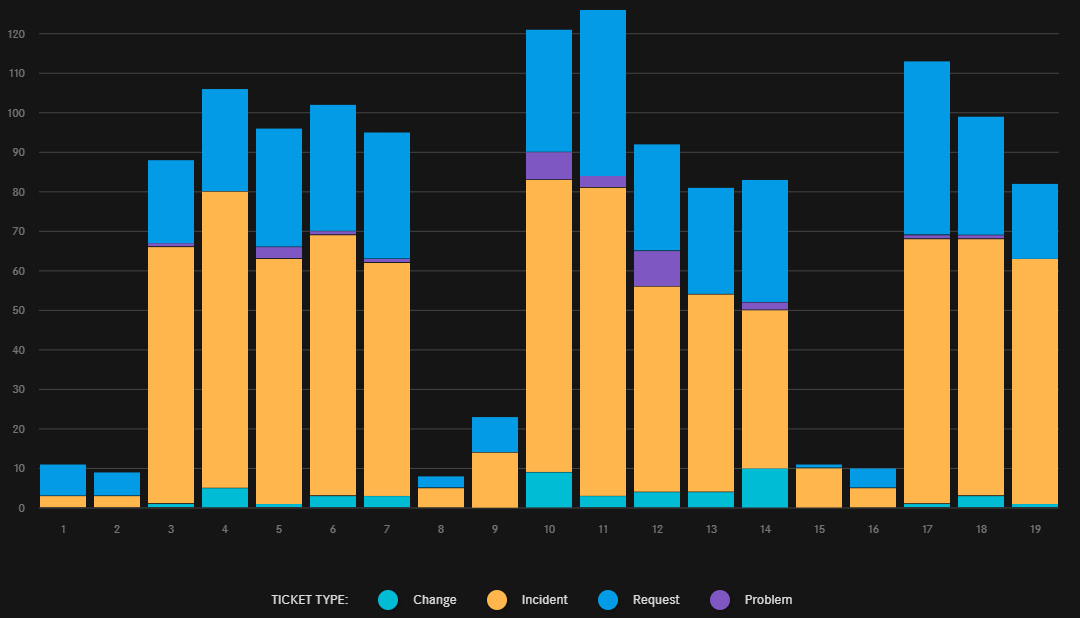
\includegraphics[
  width=400px,
  keepaspectratio,
]{dashboard1}

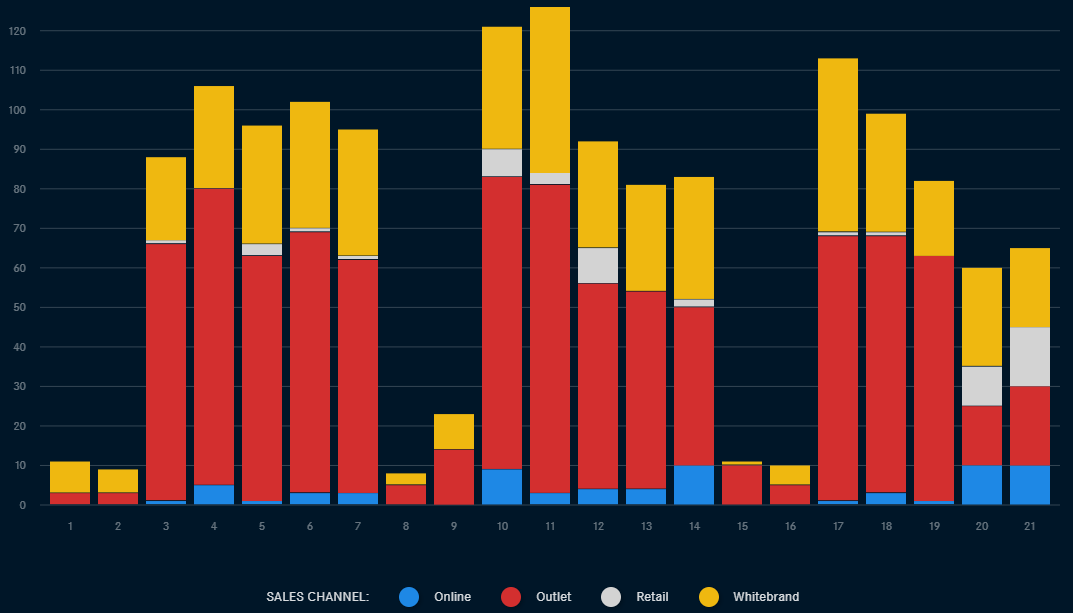
\includegraphics[
  width=400px,
  keepaspectratio,
]{dashboard2}
\end{center}
Colors and Ticket type names can be changed, it will be explained lately.
\newpage %% Page break
\noindent %% No indent first paragraph
In the right part of the main page (If you are in desktop version) or in the bottom part (If you are in mobile version). There are 4 summary tables with monthly information:
\begin{center} %% Images centered
	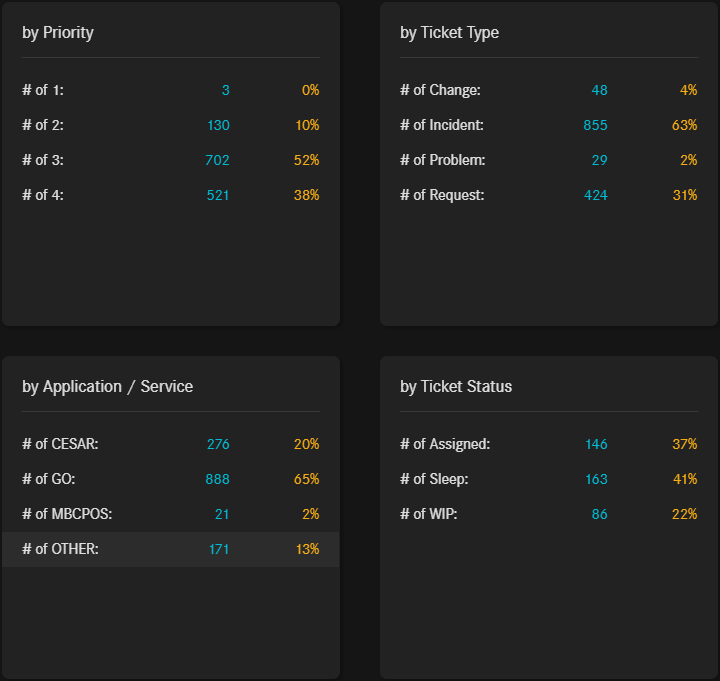
\includegraphics[
	  height=300px,
	  keepaspectratio,
	]{table1}
   
	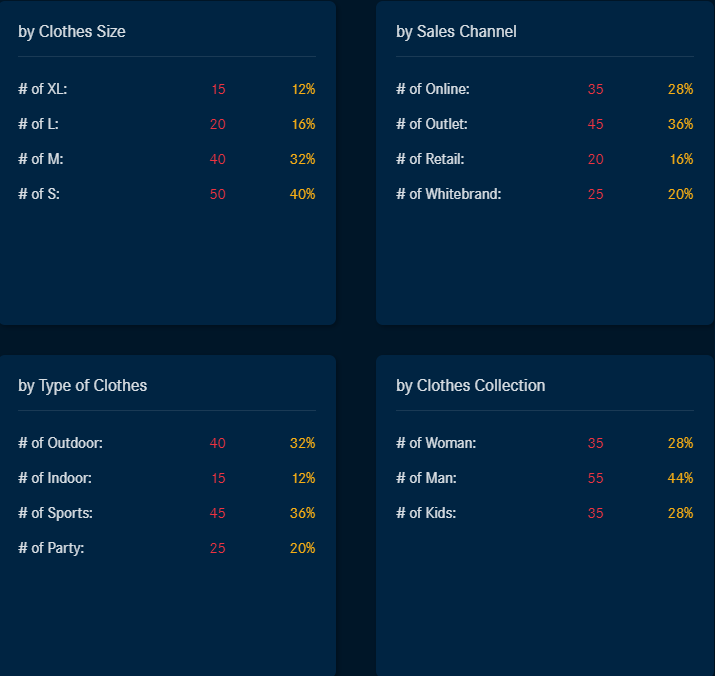
\includegraphics[
	  height=300px,
	  keepaspectratio,
	]{table2}
	\end{center}
We can see the total the total of each month and the percentage of each one
\newpage %% Page break
\section{Prepare Skinning} %% Second Section
Below, there is an image with a screenshot of the dashboard
\begin{center} %% Image Centered
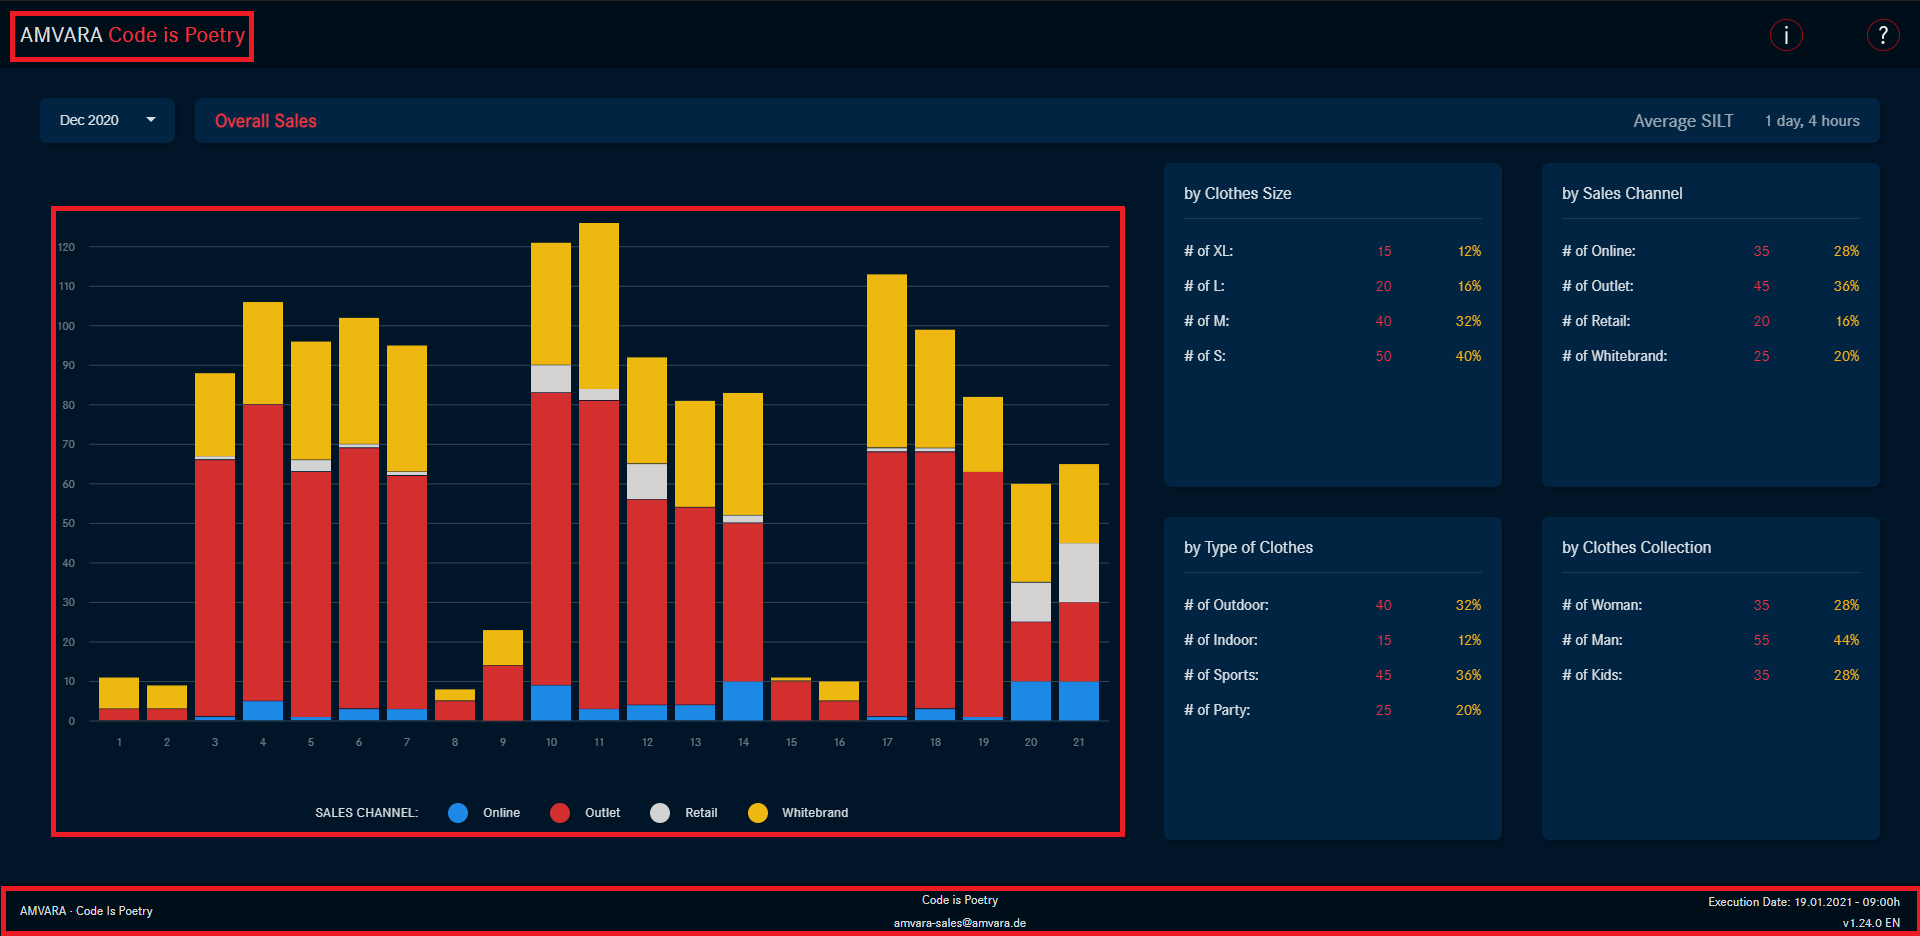
\includegraphics[
  width=400px,
  keepaspectratio,
]{principal}
\end{center}

\section{Introducing Data} %% Section three \_ \_ of filename.csv needed to print _
The data insertion or edition is done by editing the file Mobile\_List\_Chart.csv (Located in .src/assets/reports/), it's mandatory to use the same name in the ticket type column 
inside the csv and in the colorscheme inside config.json (Located in .src/assets/). If not, when clicking in the bar chart data will not be displayed correctly.\par

\end{document} %% End of document
